\documentclass[11pt,a4paper]{article}

% ===================== Codificación y fuentes =====================
\usepackage[utf8]{inputenc}
\usepackage[T1]{fontenc}

% ===================== Página y utilidades ========================
\usepackage[left=2.5cm,right=2.5cm,top=2.5cm,bottom=2.5cm]{geometry}
\usepackage{array}
\usepackage{enumitem}
\usepackage{graphicx}
\usepackage{float}
\usepackage{xcolor}
\usepackage{titlesec}
\usepackage{fancyhdr}
\usepackage[most]{tcolorbox}
\usepackage{hyperref}
\usepackage{booktabs}

% ===================== Etiquetas en español (sin babel) ===========
\renewcommand{\contentsname}{Índice}
\renewcommand{\figurename}{Figura}
\renewcommand{\tablename}{Tabla}
\renewcommand{\refname}{Bibliografía}

% ===================== Escala de grises (sin color) ================
\definecolor{negro}{RGB}{0,0,0}
\definecolor{gris}{RGB}{90,90,90}
\definecolor{grisclaro}{RGB}{150,150,150}
\definecolor{fillgray}{RGB}{175,175,175}

% ===================== Hipervínculos (negro) =======================
\hypersetup{colorlinks=true, linkcolor=negro, urlcolor=negro, citecolor=negro}

% ===================== Estilo de títulos ===========================
\titleformat{\section}{\large\bfseries\color{negro}}{\thesection.}{0.5em}{}
\titleformat{\subsection}{\normalsize\bfseries\color{negro}}{\thesubsection}{0.5em}{}
\titlespacing*{\section}{0pt}{1.4em}{0.4em}
\titlespacing*{\subsection}{0pt}{1.0em}{0.3em}

% ===================== Pie de página ===============================
\pagestyle{fancy}
\fancyhf{}
\fancyfoot[L]{\footnotesize\color{gris}Magíster en Ciencia de Datos e Inteligencia Artificial}
\fancyfoot[R]{\footnotesize\color{gris}\thepage}
\renewcommand{\headrulewidth}{0pt}
\renewcommand{\footrulewidth}{0.4pt}

% ===================== Comandos del docente ========================
\newcommand{\guia}[1]{{\small\itshape\color{gris}#1}\par\vspace{0.15em}}
\newcommand{\resp}{{\footnotesize\itshape\color{fillgray}[\,Desarrollen aquí\,]}\par\vspace{1.1em}}

% Caja de información de la evaluación (escala de grises):
\newtcolorbox{infobox}[1][Información de la evaluación]{colback=black!3,colframe=negro,
  fonttitle=\bfseries,coltitle=white,title={#1},boxrule=0.6pt,arc=1pt,
  left=8pt,right=8pt,top=6pt,bottom=6pt,breakable}

% Caja de conexión con evaluaciones previas (gris, sin color):
\newtcolorbox{conexionbox}[1][Conexión con evaluaciones anteriores]{colback=black!6,colframe=gris,
  fonttitle=\bfseries,coltitle=white,title={#1},boxrule=0.6pt,arc=1pt,
  left=8pt,right=8pt,top=6pt,bottom=6pt,breakable}

% ===================== Datos del grupo (COMPLETAR) ==================
\newcommand{\proyTitulo}{Predicción de riesgo de enfermedad coronaria a 10 años}
\newcommand{\proyIntegrantes}{Felipe Díaz Toro, Pablo Ríos Passteni, Guillermo Subiabre Chacón, Ninoska Yévenes Hernández}
\newcommand{\proyDataset}{Framingham Heart Study (Riesgo Cardiovascular)}
\newcommand{\proyDocente}{Jean Paul Maidana}
\newcommand{\proyFecha}{21/10/2026}
\newcommand{\proyRepo}{\url{https://github.com/fdiaztoro/proyecto-grupo3-mcdi501}}

\setlength{\parindent}{0pt}
\setlength{\parskip}{0.35em}

\begin{document}
\pagenumbering{gobble}

\thispagestyle{empty}
\begin{center}
\vspace*{1.0cm}

\includegraphics[height=4.4cm]{logo_unab.png}\\[1.3cm]

{\footnotesize\color{gris}\MakeUppercase{Magíster en Ciencia de Datos e Inteligencia Artificial}}\\[0.15cm]
{\footnotesize\color{grisclaro}MCDI501: Estadística Computacional para la Toma de Decisiones}\\[2.0cm]

{\Large\bfseries\color{negro} Evaluación Sumativa 3}\\[0.45cm]
{\large\color{negro} Modelamiento Predictivo Integrado}\\[1.0cm]

{\small\itshape\color{gris} Informe técnico grupal \textperiodcentered\ 60\,\%}
\end{center}

\vspace{1.6cm}

\begin{flushleft}
\setlength{\extrarowheight}{5pt}
\begin{tabular}{@{}>{\bfseries\color{negro}}l @{\hspace{0.6em}} p{0.72\linewidth}@{}}
Título del proyecto: & \proyTitulo \\
Integrantes:         & \proyIntegrantes \\
Dataset:             & \proyDataset \\
Docente:             & \proyDocente \\
Fecha:               & \proyFecha \\
Repositorio GitHub:  & \proyRepo \\
\end{tabular}
\end{flushleft}

\clearpage
\pagenumbering{arabic}

\section*{Resumen ejecutivo}
Este informe integra S1, S2 y F2 en un modelo predictivo del riesgo de enfermedad coronaria (CHD) a 10 años, con 4.238 participantes del estudio de Framingham (15,2\,\% con CHD; Dileep, 2019). La glucosa, que falta en el 9,16\,\% de los registros, se imputó con una regresión lineal múltiple (R$^2$ = 0,41; error de validación cruzada 23\,\% menor que el de la mediana) bajo un supuesto MAR, y se comparó con eliminar los casos y con imputar la mediana. Se ajustaron tres modelos logísticos con criterios de selección distintos: el de F2 (edad, sistólica, sexo, cigarrillos por día y glucosa, 5 variables), una selección hacia adelante por AIC (8 variables) y un modelo reducido sin glucosa (4 variables, para no depender de la única variable imputada). El de F2 tiene el mejor AUC en test (0,703) y fue elegido como modelo final. Ponderar las clases (peso 3,29 para los casos) sube el recall de 4,7\,\% a 60,1\,\% sin alterar el AUC. El bootstrap (2.000 remuestras) confirma que ningún coeficiente cruza el cero, y la estrategia de imputación no cambia las conclusiones. La limitación principal es la capacidad discriminativa moderada (AUC $\approx$ 0,70), que impide usar el modelo como herramienta de diagnóstico individual.

\section{Introducción y progresión S1 $\to$ S2 $\to$ S3}
La enfermedad coronaria es una de las principales causas de muerte en el mundo. Con la copia versionada del estudio de Framingham (Dileep, 2019; huella SHA-256 verificada en cada evaluación) buscamos predecir si una persona desarrollará CHD en 10 años a partir de sus factores de riesgo. Solo el 15,2\,\% de los participantes la desarrolla, por lo que la clase de interés es minoritaria. La Tabla~\ref{tab:prog} resume qué heredó este trabajo de las evaluaciones previas.

\begin{table}[H]
\centering\small
\caption{Qué aporta cada fase a la siguiente.}\label{tab:prog}
\begin{tabular}{@{}p{0.07\linewidth}p{0.42\linewidth}p{0.43\linewidth}@{}}
\toprule
\textbf{Fase} & \textbf{Hallazgo} & \textbf{Uso en S3} \\
\midrule
S1 & Edad ($r=0,225$) y sistólica ($r=0,216$) son las más asociadas a CHD; faltantes en 7 variables, glucosa con 9,16\,\%; valores extremos plausibles & Base de la selección de variables y de los predictores de la imputación; referencia del mecanismo de faltantes \\
S2 & Correlaciones de edad [0,197; 0,254] y sistólica [0,183; 0,250] estables por bootstrap; diastólica e hipertensión colineales con la sistólica ($r=0,78$ y $0,70$); cinco observaciones influyentes & Una sola variable de presión en los tres modelos; revisión de influyentes \\
F2 & Modelo de 5 variables: AUC 0,703, pero recall de solo 4,7\,\% con umbral 0,5 & Punto de partida: se corrige el recall con ponderación de clases \\
\bottomrule
\end{tabular}
\end{table}

\section{Manejo inteligente de datos faltantes}
\subsection{Referencia a S1 y mecanismo de falta}
Siete variables tienen faltantes: glucosa 388 (9,16\,\%), educación 105 (2,48\,\%), medicación antihipertensiva 53 (1,25\,\%), colesterol 50 (1,18\,\%), cigarrillos por día 29 (0,68\,\%), IMC 19 (0,45\,\%) y frecuencia cardíaca 1; en total, 582 personas (13,7\,\%) tienen al menos un dato faltante. La glucosa es la más afectada y la que analizamos en detalle. En S1, su falta no se asoció con el desenlace ($\chi^2=1,58$; $p=0,21$), lo que por sí solo no dice nada sobre el mecanismo. Aquí comparamos, con las variables sin faltantes, a quienes tienen la glucosa registrada con quienes no (Tabla~\ref{tab:meca}).

\begin{table}[H]
\centering\small
\caption{Glucosa faltante frente a observada, en variables sin faltantes.}\label{tab:meca}
\begin{tabular}{@{}lrrr@{}}
\toprule
\textbf{Variable} & \textbf{Faltante} & \textbf{Observada} & \textbf{$p$} \\
\midrule
Sexo masculino        & 29,6\,\% & 44,3\,\% & $<0,0001$ \\
Diabetes              & 1,0\,\%  & 2,7\,\%  & 0,065 \\
Fumador actual        & 52,8\,\% & 49,1\,\% & 0,173 \\
Edad (media)          & 49,0     & 49,6     & 0,148 \\
Presión sistólica (media) & 131,4 & 132,5   & 0,346 \\
\bottomrule
\end{tabular}
\end{table}

La única diferencia clara es el sexo: la glucosa falta más en mujeres. Una regresión logística del indicador de falta confirma el patrón (ser hombre reduce las odds de falta a la mitad, OR $\approx$ 0,50), aunque explica muy poco (pseudo R$^2$ = 0,017). Se descarta entonces un mecanismo completamente aleatorio (MCAR) y se adopta como \textbf{supuesto de trabajo MAR}: la falta depende de variables observadas, principalmente el sexo. Los tests solo pueden rechazar MCAR; no pueden demostrar MAR, porque un mecanismo MNAR no se distingue desde lo observado (Little y Rubin, 2019). Esto obliga a incluir el sexo como predictor de la imputación.

\subsection{Imputación mediante regresión lineal múltiple}
Para no contaminar la evaluación, la partición 70/30 estratificada por \texttt{TenYearCHD} (2.966 en train y 1.272 en test; prevalencia 15,21\,\% y 15,17\,\%) se hace \emph{antes} de imputar, y el modelo se ajusta solo con los 2.680 casos de train con glucosa registrada. Los predictores se eligieron entre las variables sin faltantes por su correlación con la glucosa y su respaldo de S2: diabetes ($r=0,635$), presión sistólica (0,135), edad (0,112), sexo (por el mecanismo) y fumador actual (por su asociación débil con la falta). Se omiten diastólica e hipertensión por colinealidad con la sistólica. La variable objetivo no se usa jamás.

El modelo explica el 41\,\% de la varianza (R$^2$ = 0,408; error típico 18,4\,mg/dL), pero casi todo viene de la diabetes (+89\,mg/dL); la sistólica aporta apenas 0,06\,mg/dL por mmHg y edad, sexo y tabaquismo no son significativos. En validación cruzada de 5 pliegues, su error (18,6\,mg/dL) es 23\,\% menor que el de imputar la mediana (24,2\,mg/dL), sin señales de sobreajuste. Los residuos son asimétricos (asimetría 2,14) y su varianza es mayor en diabéticos, de modo que los valores $p$ del modelo son poco confiables, aunque las predicciones promedio que necesitamos sí lo son. Se imputaron 388 valores (286 en train y 102 en test). Como casi todos los imputados son personas sin diabetes, reciben valores cercanos a 80\,mg/dL (media 80,3; desv. est. 9,3, frente a 23,9 en la glucosa observada): la imputación determinista comprime la variabilidad. Una variante con ruido residual la recupera (22,9), pero exagera las colas, por lo que se usa solo como análisis de sensibilidad.

\begin{figure}[H]
\centering
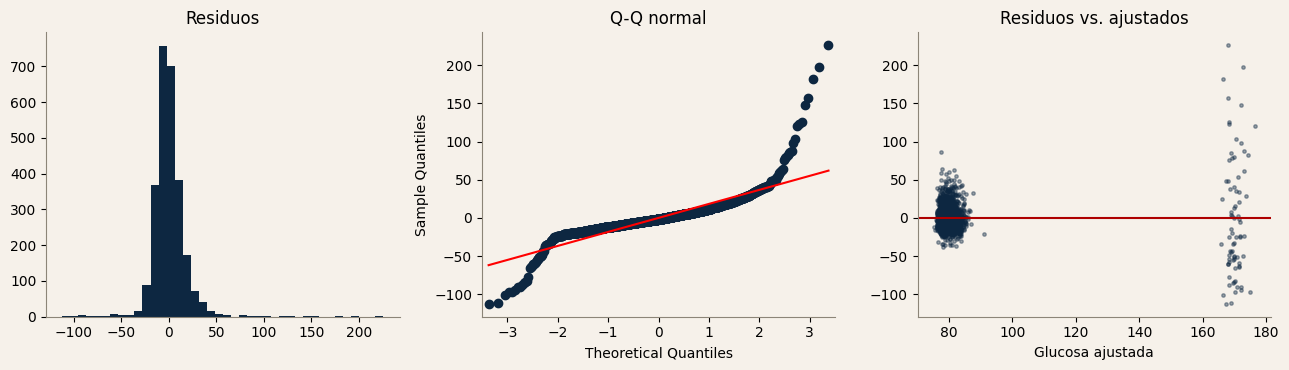
\includegraphics[width=\linewidth]{figuras/fig_imputacion_residuos.png}
\caption{Residuos del modelo de imputación: histograma, gráfico Q-Q normal y residuos frente a valores ajustados. Los valores ajustados forman dos nubes (sin y con diabetes) y los residuos tienen cola derecha larga.}\label{fig:resimp}
\end{figure}

\subsection{Comparación de estrategias de imputación}
Comparamos la eliminación de casos, la imputación por la mediana y la imputación por regresión (con la variante con ruido) en tamaño de muestra, distribución y preservación de las correlaciones de S1, sobre el conjunto de entrenamiento (Tabla~\ref{tab:comp}, Figura~\ref{fig:glu}).

\begin{table}[H]
\centering\small
\caption{Comparación de estrategias de imputación de la glucosa (entrenamiento).}\label{tab:comp}
\begin{tabular}{@{}lrrrr@{}}
\toprule
 & \textbf{Elimin.} & \textbf{Mediana} & \textbf{Regresión} & \textbf{Reg.+ruido} \\
\midrule
$n$                          & 2.680 & 2.966 & 2.966 & 2.966 \\
\% hombres                   & 44,4  & 43,3  & 43,3  & 43,3 \\
Prevalencia CHD (\%)         & 15,52 & 15,21 & 15,21 & 15,21 \\
Desv. est. de la glucosa     & 23,85 & 22,71 & 22,86 & 23,77 \\
Asimetría                    & 5,74  & 6,07  & 5,97  & 5,65 \\
$r$ glucosa--diabetes        & 0,635 & 0,623 & 0,642 & 0,615 \\
$r$ glucosa--sistólica       & 0,135 & 0,129 & 0,137 & 0,135 \\
$r$ glucosa--CHD             & 0,120 & 0,116 & 0,121 & 0,114 \\
\bottomrule
\end{tabular}
\end{table}

\begin{figure}[H]
\centering
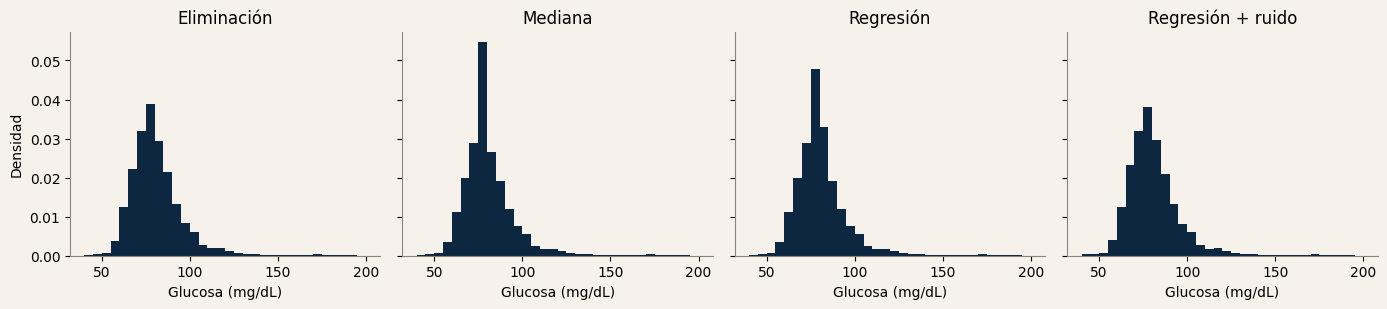
\includegraphics[width=\linewidth]{figuras/fig_glucosa_estrategias.png}
\caption{Distribución de la glucosa según la estrategia (entrenamiento).}\label{fig:glu}
\end{figure}

Como solo el 9,6\,\% de la glucosa de train se imputó, las diferencias son pequeñas. Eliminar pierde 286 personas y sube levemente el porcentaje de hombres, coherente con el mecanismo. La mediana crea un pico artificial en 78\,mg/dL y debilita las correlaciones. La regresión las conserva (diferencias menores a 0,01) y mantiene la relación con CHD, que no entró en la imputación (0,121 frente a 0,120). Parte del buen resultado con diabetes, sistólica y edad es esperable, porque la regresión las usa. La variante con ruido es la que más las diluye. \textbf{Se elige la regresión determinista}: conserva toda la muestra, preserva las relaciones de S1 y no depende del azar.

\section{Clasificación mediante regresión logística}
\subsection{Preparación de datos}
Sobre la glucosa imputada, el resto de los faltantes menores se rellena con la mediana de train; en cigarrillos por día se usa la de los \emph{fumadores} (20), porque los 29 faltantes son todos fumadores actuales y la mediana general es 0. La regla de Tukey que se aplicó en F2 marcó valores extremos en sistólica (3,0\,\%), glucosa (4,9\,\%) y cigarrillos (0,3\,\%); S1 y F2 concluyeron que los de sistólica y cigarrillos son clínicamente plausibles y no los trataron, decisión que mantenemos. La glucosa es la única donde S2 recomendó acotar la cola, lo que hacemos al percentil 99 de train (187,1\,mg/dL). Los 14 candidatos se estandarizan con la media y la desviación de train (Pedregosa et~al., 2011). Educación es la única variable categórica del dataset (ordinal, 4 niveles) y se excluye en vez de codificarse, por tener faltantes propios y una asociación débil con el desenlace ($r=-0,054$); las demás variables usadas son binarias y no requieren codificación adicional. Por la estandarización, todo odds ratio (OR) se lee por cada desviación estándar del predictor.

\subsection{Tres modelos con distintos criterios de selección}
Los tres se ajustan con \texttt{statsmodels} (Seabold y Perktold, 2010), siguiendo la estructura que pidió el profesor en la retroalimentación de F2 (``ajusten 3 regresiones logísticas, una con estas 5 variables, otra por stepwise según AIC y una reducida''): el \textbf{Modelo 1} reutiliza las cinco variables de F2 (edad, sistólica, sexo, cigarrillos por día y glucosa), ya justificadas con evidencia de S1 y S2; el \textbf{Modelo 2} es una selección hacia adelante por AIC sobre los 14 candidatos; el \textbf{Modelo 3}, reducido, elimina deliberadamente la glucosa del Modelo 1 (la única de las cinco variables con valores imputados, 9,2\,\%), para tener una alternativa que no dependa de ningún dato imputado.

\begin{table}[H]
\centering\small
\caption{Comparación de los tres modelos en test (AUC sin ponderar; recall y F1 con modelos ponderados, umbral 0,5).}\label{tab:mod}
\begin{tabular}{@{}p{0.27\linewidth}rrrrrr@{}}
\toprule
\textbf{Modelo} & \textbf{Var.} & \textbf{AIC} & \textbf{BIC} & \textbf{AUC} & \textbf{Recall} & \textbf{F1} \\
\midrule
1. Guiado por S1/S2 (como F2)          & 5 & 2.243,3 & 2.279,3 & 0,703 & 0,601 & 0,352 \\
2. Hacia adelante por AIC              & 8 & 2.233,7 & 2.287,7 & 0,699 & 0,596 & 0,349 \\
3. Reducido (sin glucosa)              & 4 & 2.254,0 & 2.283,9 & 0,701 & 0,617 & 0,356 \\
\bottomrule
\end{tabular}
\end{table}

El Modelo 2 incorpora, en este orden, edad, sistólica, cigarrillos, glucosa y sexo (las cinco del Modelo 1, que un algoritmo que no las conocía eligió primero), y luego antecedente de ACV, colesterol y medicación, con efectos pequeños (OR 1,09 a 1,13) y $p$ en el borde de la significancia (0,008 a 0,045). Antes de construir el Modelo 3 probamos si el AIC/BIC puro justifica reducir el Modelo 1: eliminar cualquiera de sus cinco variables \textbf{empeora} el AIC (sube de 2.243,3 a entre 2.253,6 y 2.344,4 según cuál se saque), así que el criterio estadístico no reduce el modelo por sí solo. Por eso el Modelo 3 reduce por un criterio distinto —calidad del dato, no ajuste estadístico—: sin la glucosa, el AIC sube solo 10,7 puntos y las cuatro variables restantes siguen siendo significativas. Los tres modelos quedan así genuinamente distintos (5, 8 y 4 variables). El modelo completo (14 variables) no mejora al Modelo 1 en AIC (2.243,3) y tiene el peor BIC (2.333,2).

\subsection{Ponderación de clases y desempeño}
Con umbral 0,5, el modelo de F2 detectaba solo el 4,7\,\% de los casos. Ponderamos cada observación con el inverso de la frecuencia de su clase (3,29 para los casos y 0,59 para los demás; igual que \texttt{class\_weight='balanced'} y coherente con el $\approx$3,3 que prevé la prevalencia de 15,2\,\%). Las curvas ROC de los tres modelos se muestran en la Figura~\ref{fig:roc}.

\begin{figure}[H]
\centering
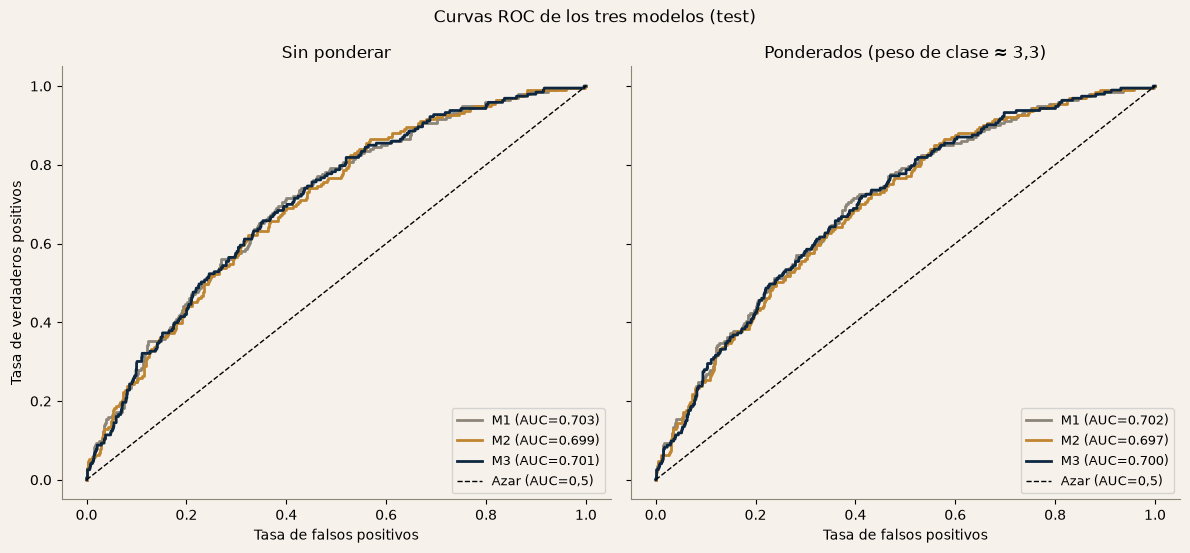
\includegraphics[width=0.92\linewidth]{figuras/fig_roc.png}
\caption{Curvas ROC de los tres modelos en el conjunto de prueba, sin ponderar (izquierda) y ponderados (derecha).}\label{fig:roc}
\end{figure}

\begin{table}[H]
\centering\small
\caption{Modelo final (Modelo 1) en entrenamiento y prueba, sin ponderar y ponderado.}\label{tab:conf}
\begin{tabular}{@{}llrrrrrr@{}}
\toprule
\textbf{Ajuste} & \textbf{Conjunto} & \textbf{VN} & \textbf{FP} & \textbf{FN} & \textbf{VP} & \textbf{Accuracy} & \textbf{Recall} \\
\midrule
Sin ponderar & Train & 2.500 & 15  & 414 & 37  & 0,855 & 0,082 \\
Sin ponderar & Test  & 1.066 & 13  & 184 & 9   & 0,845 & 0,047 \\
Ponderado    & Train & 1.700 & 815 & 137 & 314 & 0,679 & 0,696 \\
Ponderado    & Test  & 729   & 350 & 77  & 116 & 0,664 & 0,601 \\
\bottomrule
\end{tabular}
\end{table}

La ponderación detecta 116 de los 193 casos del test (de 9 antes) a costa de más falsos positivos (precision de 25\,\%) y menor accuracy, que ya no es el espejismo de predecir siempre ``sin CHD'' (el clasificador trivial acierta 84,8\,\%). El AUC no se mueve (0,703 a 0,702): la ponderación solo cambia el punto de corte sobre la misma curva. El recall baja algo más de train a test (69,6\,\% a 60,1\,\%) que el AUC (0,738 a 0,702), una señal de sobreajuste leve en el punto de corte, no en la capacidad de ordenar por riesgo. Ponderados, el Modelo 1 llega a AUC 0,702, el Modelo 2 a 0,697 (mejora el entrenamiento a 0,744 sin mejorar el test, señal de sobreajuste leve por sus tres variables adicionales) y el Modelo 3 a 0,700, con mejor recall (61,7\,\%) y F1 (0,356) que el Modelo 1. \textbf{El modelo final es el Modelo 1, ponderado}: tiene el mejor AUC de los tres —la métrica que no depende del umbral, y por eso la más robusta para comparar— y usa la glucosa, un marcador clínico relevante que imputamos con un método validado (Sección 2); no vemos necesario descartarla solo por su incertidumbre de imputación. El Modelo 3 queda documentado como alternativa competitiva y más simple si se prioriza no depender de datos imputados. El AUC de 0,70 es aceptable, no alto (Hosmer et~al., 2013).

\subsection{Estabilidad mediante bootstrap}
Se aplicó bootstrap no paramétrico al modelo final: 2.000 remuestras de las filas de train, recalculando en cada una el peso de clase y reajustando el modelo, con IC percentil al 95\,\% (Efron y Tibshirani, 1993), comparado con el IC de Wald tradicional (Tabla~\ref{tab:boot}). Todas las remuestras convergieron.

\begin{table}[H]
\centering\small
\caption{OR por desviación estándar del modelo final, con IC al 95\,\% bootstrap y de Wald.}\label{tab:boot}
\begin{tabular}{@{}lrcc@{}}
\toprule
\textbf{Variable} & \textbf{OR} & \textbf{IC bootstrap} & \textbf{IC Wald} \\
\midrule
Edad                 & 1,90 & [1,70; 2,14] & [1,73; 2,08] \\
Presión sistólica    & 1,47 & [1,32; 1,64] & [1,35; 1,59] \\
Cigarrillos por día  & 1,34 & [1,20; 1,50] & [1,23; 1,46] \\
Sexo masculino       & 1,20 & [1,06; 1,35] & [1,10; 1,30] \\
Glucosa              & 1,16 & [1,05; 1,28] & [1,08; 1,25] \\
\bottomrule
\end{tabular}
\end{table}

Ningún IC bootstrap incluye el 1: los cinco parámetros son estables. Los menos estables son \textbf{glucosa y sexo}, cuyos límites inferiores están más cerca de 1 (en coeficiente, 0,052 y 0,057). Los IC bootstrap son más anchos que los de Wald en los cinco predictores, porque Wald supone normalidad asintótica y no recoge la incertidumbre de recalcular el peso de clase. Ningún parámetro cambia de signo ni de significancia entre ambos métodos. Usamos 2.000 y no 10.000 remuestras (S2) porque cada una reajusta un modelo ponderado.

\subsection{Diagnóstico de supuestos}
Sobre el modelo final sin ponderar (Modelo 1; la ponderación no cambia la especificación): el \textbf{VIF} está entre 1,03 y 1,23, sin multicolinealidad; si se agregaran diastólica e hipertensión, el de la sistólica subiría de 1,20 a 3,69 (coincide con el máximo de 3,71 que reportó el profesor en su retroalimentación de F2), lo que respalda conservar una sola variable de presión. La \textbf{linealidad en el logit} (Box y Tidwell, 1962) se cumple para sistólica ($p=0,27$), cigarrillos (0,71) y glucosa (0,098), pero no del todo para la \textbf{edad} ($p=0,011$, que sobrevive a corregir por las cuatro pruebas); no se corrige para conservar la interpretación del OR y queda como limitación. De las observaciones influyentes de S2, solo la 481 y la 2197 caen en el train de S3 y ambas quedan bajo el umbral $4/n$ (Cook $=0,00077$ y $0,00121$, frente a $0,00135$); el máximo global es 0,0096, muy lejos de 1. Los residuos no muestran patrones preocupantes (Figura~\ref{fig:diag}).

\begin{figure}[H]
\centering
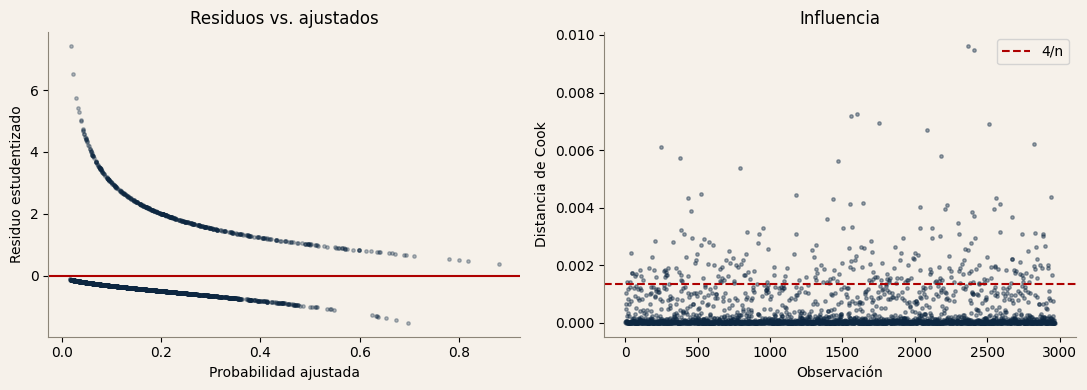
\includegraphics[width=0.9\linewidth]{figuras/fig_diagnostico.png}
\caption{Diagnóstico del modelo final (Modelo 1): residuos estudentizados frente a la probabilidad ajustada (izquierda) y distancia de Cook por observación (derecha; línea roja, umbral $4/n$).}\label{fig:diag}
\end{figure}

\section{Análisis comparativo del impacto de la imputación}
Reajustamos el modelo final con las tres versiones del dataset, desde la misma partición; la eliminación quita las filas sin glucosa observada de ambos conjuntos, y cada estrategia re-estandariza y reajusta su modelo ponderado (Tabla~\ref{tab:imp}).

\begin{table}[H]
\centering\small
\caption{Modelo final con cada estrategia de imputación.}\label{tab:imp}
\begin{tabular}{@{}lrrrrrrr@{}}
\toprule
\textbf{Estrategia} & \textbf{$n$ train} & \textbf{$n$ test} & \textbf{AUC test} & \textbf{Accuracy} & \textbf{Recall} & \textbf{OR edad} & \textbf{OR glucosa} \\
\midrule
Eliminación & 2.680 & 1.170 & 0,703 & 0,667 & 0,601 & 1,95 & 1,15 \\
Mediana     & 2.966 & 1.272 & 0,702 & 0,661 & 0,601 & 1,89 & 1,15 \\
Regresión   & 2.966 & 1.272 & 0,702 & 0,664 & 0,601 & 1,90 & 1,16 \\
\bottomrule
\end{tabular}
\end{table}

La estrategia de imputación casi no cambia las conclusiones: AUC, recall y odds ratios son prácticamente idénticos. La diferencia real es el tamaño de muestra: eliminar pierde 388 personas (286 en train y 102 en test), reduce la precisión y sesga levemente la composición por sexo; además, su test es más chico, por lo que sus métricas no son estrictamente comparables. Se confirma la imputación por regresión como la opción por defecto. Con tan pocos valores imputados, las tres no se distinguen, y con una tasa de faltantes mayor la brecha probablemente sería mayor.

\section{Discusión y conclusiones}
\textbf{Progresión.} S1 señaló edad y presión sistólica y describió faltantes y extremos; S2 validó esas correlaciones y detectó la colinealidad de la presión; F2 las convirtió en un modelo de 5 variables cuyo recall era casi nulo, y el profesor lo calificó con 96/96, pidiendo para S3 exactamente estos tres modelos (uno con esas 5 variables, uno por stepwise AIC y uno reducido). S3 trató la glucosa con un método más honesto que la mediana, construyó los tres modelos pedidos (el de 5 variables de F2 resultó ganador por AUC; el reducido, de 4 variables sin glucosa, quedó como alternativa competitiva) y corrigió el recall ponderando las clases. El modelo final detecta el 60,1\,\% de los casos del test con un AUC de 0,70, es estable al bootstrap y no tiene multicolinealidad.

\textbf{Limitaciones.} (1) El AUC de 0,70 es moderado: el modelo ordena razonablemente el riesgo, pero no separa bien a los casos de los no casos, y con precision de 25\,\% no sirve como diagnóstico individual. (2) El MAR de la glucosa es un supuesto no verificable. (3) La imputación, aunque mejor que la mediana, comprime la variabilidad de la glucosa. (4) La edad presenta una no linealidad leve no corregida. (5) Se usó un único logístico lineal y una sola partición, con 193 casos en el test.

\textbf{Recomendaciones.} Explorar un término no lineal para la edad (cuadrático o \emph{splines}); elegir el umbral de decisión según el costo relativo de un falso negativo frente a uno falso positivo, en vez de fijarlo en 0,5; usar validación cruzada como diagnóstico adicional de estabilidad entre los tres modelos (sin reemplazar la partición 70/30, que se mantiene como evaluación principal); y comparar contra un modelo no lineal para medir lo que se pierde por restringirse a lo lineal.

\section*{Bibliografía (APA 7)}
\begin{list}{}{\leftmargin=1.5em \itemindent=-1.5em \itemsep=0.25em \parsep=0pt}\small\raggedright
\item Box, G. E. P., \& Tidwell, P. W. (1962). Transformation of the independent variables. \textit{Technometrics, 4}(4), 531--550.
\item Dileep. (2019). \textit{Logistic regression to predict heart disease} (Versión 1) [Conjunto de datos]. Kaggle. \url{https://www.kaggle.com/datasets/dileep070/heart-disease-prediction-using-logistic-regression}
\item Efron, B., \& Tibshirani, R. J. (1993). \textit{An introduction to the bootstrap}. Chapman \& Hall.
\item Hosmer, D. W., Lemeshow, S., \& Sturdivant, R. X. (2013). \textit{Applied logistic regression} (3.\textsuperscript{a} ed.). Wiley. \url{https://doi.org/10.1002/9781118548387}
\item Little, R. J. A., \& Rubin, D. B. (2019). \textit{Statistical analysis with missing data} (3.\textsuperscript{a} ed.). Wiley. \url{https://doi.org/10.1002/9781119482260}
\item Pedregosa, F., Varoquaux, G., Gramfort, A., Michel, V., Thirion, B., Grisel, O., Blondel, M., Prettenhofer, P., Weiss, R., Dubourg, V., Vanderplas, J., Passos, A., Cournapeau, D., Brucher, M., Perrot, M., \& Duchesnay, É. (2011). Scikit-learn: Machine learning in Python. \textit{Journal of Machine Learning Research, 12}, 2825--2830.
\item Seabold, S., \& Perktold, J. (2010). statsmodels: Econometric and statistical modeling with Python. En S. van der Walt \& J. Millman (Eds.), \textit{Proceedings of the 9th Python in Science Conference} (pp.~92--96). \url{https://doi.org/10.25080/Majora-92bf1922-011}
\end{list}

\end{document}
